\documentclass[10pt,a4paper]{report}

% Packages
\usepackage[a4paper,margin=0.9in]{geometry} % reduce margins
\usepackage{setspace}
\usepackage{titlesec}
\usepackage{hyperref}
\usepackage{graphicx} % for images
\usepackage{caption}  % better caption control
\usepackage{lipsum}   % for dummy text (remove later)
\usepackage{enumitem}
\usepackage{amssymb} % for \checkmark symbol
\usepackage{fancyhdr}
\pagestyle{fancy}
\fancyhead[L]{CS202 Lab Assignment 1 Report}
\fancyhead[R]{Shardul Junagade}
\fancyfoot[C]{\thepage}
\usepackage{xcolor}
\usepackage{listings}
\newcommand{\command}[1]{\texttt{\textcolor{blue}{#1}}}

% Listings: consistent, readable code blocks
% Colors inspired by GitHub-like theme
\definecolor{lstbg}{HTML}{F7F7F9}
\definecolor{lstborder}{HTML}{E1E4E8}
\definecolor{lstcomment}{HTML}{6A737D}
\definecolor{lstkeyword}{HTML}{D73A49}
\definecolor{lststring}{HTML}{032F62}
\definecolor{lstnumber}{HTML}{586069}

\lstdefinestyle{cncode}{
    backgroundcolor=\color{lstbg},
    basicstyle=\ttfamily\small,
    breaklines=true,
    columns=fullflexible,
    frame=single,
    rulecolor=\color{lstborder},
    framesep=6pt,
    framerule=0.6pt,
    showstringspaces=false,
    numbers=left,
    numberstyle=\tiny\color{lstnumber},
    numbersep=10pt,
    keywordstyle=\color{lstkeyword}\bfseries,
    commentstyle=\color{lstcomment}\itshape,
    stringstyle=\color{lststring},
    tabsize=4,
    captionpos=b
}

% Default listing settings (override per-block as needed)
\lstset{style=cncode, language=Python}

% Inline code convenience macro
\newcommand{\code}[1]{\texttt{#1}}

\setlength{\parindent}{0pt}
\setlength{\parskip}{0.6em}

% Remove figure numbering
\captionsetup[figure]{labelformat=empty}

% Customize section/chapter fonts
\titleformat{\chapter}[block]{\huge\bfseries}{}{0pt}{}
\titleformat{\section}{\Large\bfseries}{\thesection}{0.4em}{} 
\titleformat{\subsection}{\large\bfseries}{\thesubsection}{0.4em}{} 

% Define custom command for images with optional caption
\usepackage{xparse}
\NewDocumentCommand{\insertimage}{O{0.8\textwidth} m o}{%
    \begin{center}
        \includegraphics[width=#1]{#2}%
        \IfValueT{#3}{\\\captionof{figure}{#3}}%
    \end{center}
}

% Front Page Info
\title{\Huge Assignment-1 \\[0.5cm] \LARGE CS 331: Computer Networks}
% \author{\Large Shardul Junagade (23110297) \\[0.1cm] \Large Rishabh Jogani (23110276) \\[0.2cm] \Large Repository: \href{https://github.com/ShardulJunagade/cn-assignment-1}{cn-assignment-1}}
\author{
    \begin{tabular}{c c}
        \Large Shardul Junagade & \Large Rishabh Jogani \\
        \large (23110297) & \large (23110276) \\
    \end{tabular} \\[0.7cm]
    \Large Repository: \href{https://github.com/ShardulJunagade/cn-assignment-1}{cn-assignment-1}
}
\date{\large \today}

\begin{document}

% Front Page
\maketitle
\newpage

% Table of Contents
\tableofcontents

\textbf{Repository:} \url{https://github.com/ShardulJunagade/cn-assignment-1}

\newpage


% % ---------- Code Snippet Template ----------
% \chapter*{Code snippet template}
% \addcontentsline{toc}{chapter}{Code snippet template}

% Use the following patterns to add code to this report. Adjust the \verb|language| option per snippet.

% \textbf{Inline:} Use \code{\textbackslash code\{...\}} for short code fragments, for example: \code{pip install -r requirements.txt}.

% \textbf{Block (with caption/label):}
% \begin{lstlisting}[language=bash, caption={Run the dpkt client (Windows PowerShell)}, label={lst:run-client}]
% # Activate venv (PowerShell) and run the dpkt client
% .\\.venv\\Scripts\\Activate.ps1
% python client_dpkt.py --pcap 3.pcap --server 127.0.0.1 --port 9999
% \end{lstlisting}

% \textbf{Python example:}
% \begin{lstlisting}[language=Python, caption={Initial Python code (example.py) with Pylint errors}, label={lst:py-example}]
% print("Hello, world!")
% \end{lstlisting}

% \textbf{Include a source file from the repo:}
% % The LaTeX file lives in latex/, so use paths relative to that folder.
% % Uncomment any of the following to include real files.
% % \lstinputlisting[language=Python, caption={Client (client_dpkt.py)}, label={lst:client-dpkt}]{../client_dpkt.py}
% % \lstinputlisting[language=Python, caption={Server (server_dpkt.py)}, label={lst:server-dpkt}]{../server_dpkt.py}
% % \lstinputlisting[language=bash, caption={Requirements file}, label={lst:reqs}]{../requirements.txt}


% ---------- Example Content ----------

\chapter{Task 1: Custom DNS Resolver}
\section{Aim}
The aim of this task was to implement a custom DNS resolver system. The objective was to parse DNS query packets from a given PCAP file, add a custom header, send them to a server for resolution based on predefined rules, and log the resolved IP addresses for reporting. This task helped us understand packet parsing, custom protocol design, and time-based routing logic.

\section{Introduction}
In this assignment, we developed a client-server system to process DNS queries captured in a PCAP file. The client parsed DNS query packets, prepended a custom header containing a timestamp and sequence ID, and sent these packets to a custom server. The server extracted the header, applied time-based routing rules to select an IP address, and responded with the resolved result. We implemented the solution using two different packet processing libraries: Scapy and dpkt, to demonstrate versatility and robustness.

The custom header format was \texttt{HHMMSSID}, where \texttt{HH} is the hour, \texttt{MM} is the minute, \texttt{SS} is the second, and \texttt{ID} is the sequence number of the DNS query. The server used this header to determine the time slot and select an IP address from a pool, as specified in a JSON rules file.

At first, we built both the client and server using the Scapy library. While Scapy was convenient for quickly inspecting packets and building DNS messages, it turned out to be too slow when processing larger PCAP files. The main reasons were: (1) Scapy decodes every field of every packet into Python objects, which is computationally heavy, (2) it stores extra metadata even when we only need the DNS question name, and (3) iterating through hundreds of thousands of packets became unreasonably slow. Because of this, we reimplemented the solution in dpkt, a much lighter and faster library. With dpkt, packet parsing became significantly quicker and better suited for large-scale PCAP analysis.

\section{Procedure}

\subsection{PCAP Parsing and DNS Query Extraction}
We first parsed the provided PCAP file to extract DNS query packets. For this, we implemented two separate clients:
\begin{itemize}
    \item \textbf{Scapy-based client (\texttt{client\_scapy.py}):}
    We used \code{rdpcap} to read the PCAP and filtered standard DNS queries (\code{qr == 0}). For each query, we extracted the domain via \code{DNSQR.qname}, skipped mDNS/service discovery (\code{.local.} and names starting with \code{\_}), built the 8-byte header, and sent a UDP payload containing \textbf{header + domain string} to the server.
    \begin{lstlisting}[language=Python, caption={Filtering DNS queries and sending header+domain}, label={lst:scapy-client}]
def build_header(seq_id: int) -> str:
    return f"{datetime.now().strftime('%H%M%S')}{seq_id:02d}"

packets = rdpcap('3.pcap')
s = socket.socket(socket.AF_INET, socket.SOCK_DGRAM)
seq_id = 0
for pkt in packets:
    if pkt.haslayer(DNS) and pkt[DNS].qr == 0:
        qname = pkt[DNSQR].qname.decode()
        if qname.endswith('.local.') or qname.startswith('_'):
            continue
        header = build_header(seq_id)  # HHMMSSID
        message = header.encode() + qname.encode()
        s.sendto(message, ("127.0.0.1", 9999))
        seq_id += 1
    \end{lstlisting}
    
    \item \textbf{dpkt-based client (\texttt{client\_dpkt.py}):}
    Used dpkt's PCAP and DNS parsing utilities:
    \begin{lstlisting}
with open(pcap_path, "rb") as f:
    pcap = dpkt.pcap.Reader(f)
    for ts, buf in pcap:
        eth = dpkt.ethernet.Ethernet(buf)
        ip = eth.data
        udp = ip.data
        if isinstance(udp, dpkt.udp.UDP) and udp.dport == 53:
            dns = dpkt.dns.DNS(udp.data)
            ...
    \end{lstlisting}
\end{itemize}

% Add output image of terminal running the client here
% \insertimage[0.8\textwidth]{../images/assignment-1/client_terminal.png}[Client terminal output]

\subsection{Custom Header Construction}
For each DNS query, we constructed an 8-byte custom header in the format \texttt{HHMMSSID}, where:
\begin{itemize}
    \item \texttt{HH}: Hour (24-hour format)
    \item \texttt{MM}: Minute
    \item \texttt{SS}: Second
    \item \texttt{ID}: Sequence number of the DNS query (starting from 00)
\end{itemize}
This header was prepended to the outbound payload. In the Scapy client, the payload was \textbf{header + domain string} (not raw DNS bytes):
\begin{lstlisting}[language=Python]
hhmmss = datetime.now().strftime("%H%M%S")
seq_id_str = f"{seq_id:02d}"
header = hhmmss + seq_id_str
payload = header.encode('ascii') + qname.encode()
\end{lstlisting}

\subsection{Client-Server Communication}
The client sent the modified packet (header + DNS query) to the server over UDP. The server was implemented in two variants:
\begin{itemize}
    \item \textbf{Scapy-based server (\texttt{server\_scapy.py}):} Used Scapy to parse incoming DNS queries and extract the domain name.
    \item \textbf{dpkt-based server (\texttt{server\_dpkt.py}):} Used dpkt for the same purpose.
\end{itemize}
We configured structured logging on the dpkt server using a shared logger module before starting the UDP loop.

Example server code (dpkt with logging):
\begin{lstlisting}[language=Python, caption={dpkt server: logging + DNS parsing}, label={lst:dpkt-server}]
setup_logging("server_dpkt")

def handle_packet(data: bytes, client_addr, sock: socket.socket, rules):
header = data[:8].decode('ascii', errors='ignore')
dns_bytes = data[8:]
    dns = dpkt.dns.DNS(dns_bytes)
    domain = dns.qd[0].name.decode() if isinstance(dns.qd[0].name, bytes) else dns.qd[0].name
    domain = domain.rstrip('.')
    resolved_ip = resolve_ip_address(rules, header)
    response = f"{header}|{domain}|{resolved_ip}"
    sock.sendto(response.encode('utf-8'), client_addr)
    logging.info(f"Responded to {client_addr}: {response}")
\end{lstlisting}



% Add output image of terminal running the server here
% \insertimage[0.8\textwidth]{../images/assignment-1/server_terminal.png}[Server terminal output]

\subsection{Server-side IP Resolution}
Upon receiving a packet, the server extracted the custom header and used the hour and sequence ID to select an IP address from a pool, according to time-based rules defined in a JSON file (\texttt{rules.json}). The rules specified different IP pool ranges and hash functions for morning, afternoon, and night slots. The logic was as follows:
\begin{lstlisting}
hour = int(header[0:2])
session_id = int(header[6:8])
if 4 <= hour <= 11:
    slot_cfg = time_rules.get("morning")
elif 12 <= hour <= 19:
    slot_cfg = time_rules.get("afternoon")
else:
    slot_cfg = time_rules.get("night")
index = ip_pool_start + (session_id % hash_mod)
\end{lstlisting}
The rules and pool configuration were as described in the assignment and the provided rules documentation.

\subsection{Running the dpkt server (\texttt{run\_server})}
The server was started by calling \texttt{run\_server(host, port, rules\_path)}. It loaded the JSON rules, bound a UDP socket, and entered a loop to receive packets and dispatch them to \texttt{handle\_packet}.

\begin{lstlisting}[language=Python, caption={Server startup: run_server()}, label={lst:run-server}]
def run_server(host: str, port: int, rules_path: str):
    rules = load_rules_from_json(rules_path)
    logging.info(f"Loaded rules from {rules_path}")
    logging.info(f"IP Pool Length: {len(rules.get('ip_pool', DEFAULT_IP_POOL))}")

    server = socket.socket(socket.AF_INET, socket.SOCK_DGRAM)
    server.bind((host, port))
    logging.info(f"DNS server (dpkt) listening on {host}:{port}")

    while True:
        data, addr = server.recvfrom(65535)
        handle_packet(data, addr, server, rules)
\end{lstlisting}


\subsection{Response and Logging}
The server responded with a plain text message in the format \texttt{header|domain|resolved\_ip}. The client received this response and logged the results in a CSV file for reporting. Both implementations (Scapy and dpkt) followed this protocol. All the terminal outputs generated during execution were also saved as log files in the repository: \url{https://github.com/ShardulJunagade/cn-assignment-1/tree/main/logs}.


\section{Results}

The system successfully parsed DNS queries from the PCAP file, sent them to the server with the custom header, and received resolved IP addresses based on the specified rules. The results were saved in CSV files (\texttt{dpkt\_dns\_report.csv} and \texttt{scapy\_dns\_report.csv}), each containing the custom header, domain name, and resolved IP address for every query.

\begin{itemize}
    \item Both Scapy and dpkt implementations produced consistent results, demonstrating the correctness of the approach.
    \item The server correctly applied time-based routing rules and handled edge cases (e.g., out-of-bounds indices).
    \item The code was modular, well-commented, and robust against malformed packets.
\end{itemize}


\textbf{Sample output (CSV):}
\begin{center}
\begin{tabular}{|c|l|c|}
\hline
\textbf{Custom header value} & \textbf{Domain name} & \textbf{Resolved IP address} \\
\textbf{(HHMMSSID)} & & \\
\hline
20464700 & netflix.com & 192.168.1.11 \\
20464701 & linkedin.com & 192.168.1.12 \\
20464702 & example.com & 192.168.1.13 \\
20464703 & google.com & 192.168.1.14 \\
20464704 & facebook.com & 192.168.1.15 \\
20464705 & amazon.com & 192.168.1.11 \\
\hline
\end{tabular}
\end{center}

\textbf{DNS Resolution Rule Example:}
\begin{itemize}
    \item If the hour is 20 (night slot), the pool start is 10, and hash mod is 5. For ID 00: $10 + (00 \% 5) = 10$ $\rightarrow$ 192.168.1.11
    \item For ID 01: $10 + (01 \% 5) = 11$ $\rightarrow$ 192.168.1.12
    \item For ID 04: $10 + (04 \% 5) = 14$ $\rightarrow$ 192.168.1.15
    \newline
    \newline
\end{itemize}

\section{References}
\begin{enumerate}[label={[\arabic*]}, itemsep=0.05em, topsep=0pt]
    \item \href{https://www.wireshark.org/docs/}{Wireshark Documentation}
    \item \href{https://scapy.readthedocs.io/en/latest/}{Scapy Documentation}
    \item \href{https://dpkt.readthedocs.io/en/latest/}{dpkt Documentation}
    \item \href{https://docs.python.org/3/library/socket.html}{Python socket — Low-level networking interface}
\end{enumerate}


% Add output image of the generated CSV/report here
% \insertimage[0.8\textwidth]{../images/assignment-1/report_csv.png}[Sample CSV output]



\chapter{Task 2:Traceroute Protocol Behavior}
\section{Aim}
The purpose of this task is to understand how the \command{traceroute} and \command{tracert} utilities work on different operating systems (Windows and macOS in this case), and to analyze its behavior using packet captures.

\section{Methodology}
\begin{enumerate}
    \item On macOS, executed \command{traceroute www.google.com}.
    \item On Windows, executed \command{tracert www.google.com}.
    \item Captured network traffic into .pcap files using \command{tcpdump} (\command{sudo tcpdump -i en0 host www.google.com -w TracerouteMac.pcap}) for macOS 
    and captured .pcap files using \command{tshark} (\command{tshark -i 5 -f "host www.google.com" -w TracertWin.pcap}) for Windows.
    \item Opened captures in Wireshark, inspected the packets, and compared results.
\end{enumerate}

\section{Terminal Output}

\insertimage[0.9\textwidth]{missing_hops.png}[MacOS terminal \command{tracert} output to www.google.com.]


\insertimage[0.9\textwidth]{windows_tracert_output.png}[Windows terminal \command{tracert} output to www.google.com.]

\section{Wireshark Output}


\insertimage[0.9\textwidth]{mac_traceroute_output.png}[macOS \command{traceroute} output to www.google.com.]


\insertimage[0.9\textwidth]{wireshark_icmp_windows.png}[Windows \command{traceroute} output to www.google.com.]

\section{Observations and Answers}

\subsection*{Q1: Protocols used by default}
\begin{itemize}
    \item \textbf{Windows tracert:} Uses \textbf{ICMP Echo Request} packets with increasing TTL.  
    \item \textbf{Linux/macOS traceroute:} Uses \textbf{UDP probes to high-numbered ports} by default, unless invoked with options like \command{-I} (ICMP) or \command{-T} (TCP).  
\end{itemize}

% \begin{figure}[h]
%     \centering
%     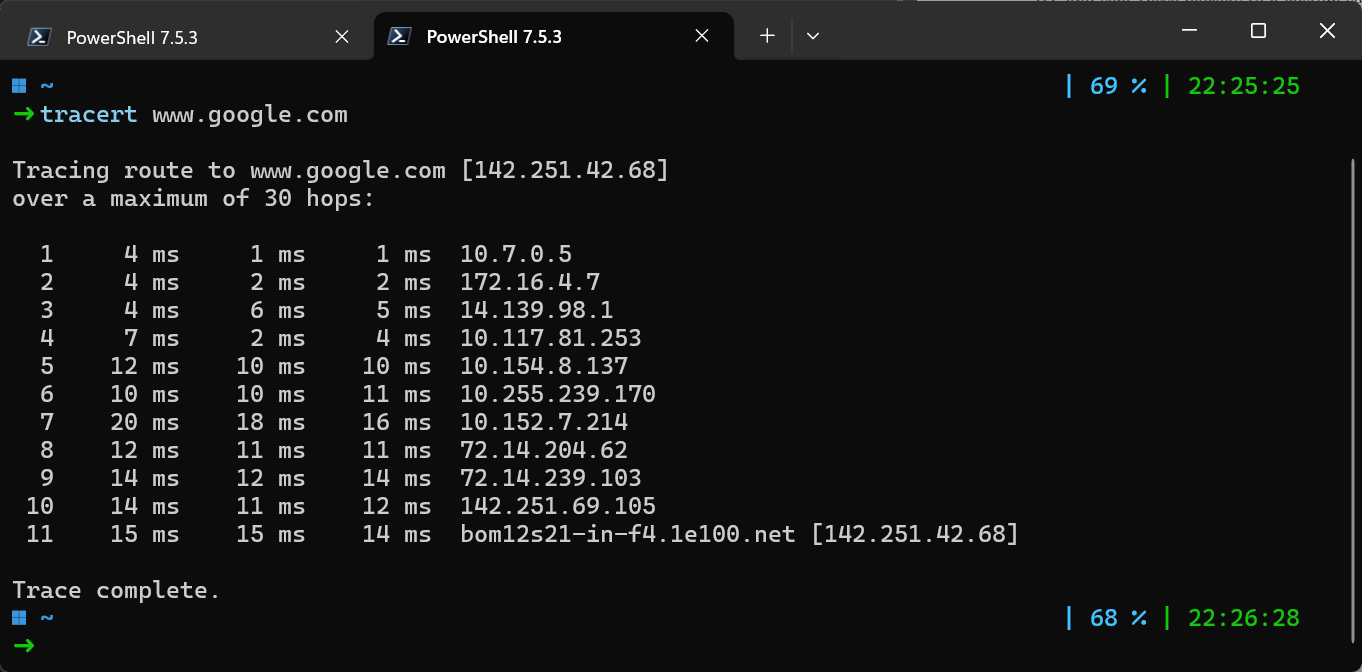
\includegraphics[width=0.9\textwidth]{windows_tracert_output.png}
    % \caption{Windows \command{tracert} output to www.google.com.}
% \end{figure}


\insertimage[0.9\textwidth]{mac_traceroute_output.png}[macOS \command{traceroute} output to www.google.com.]

\subsection*{Q2: Why might some hops show \texttt{* * *}?}
\begin{enumerate}
    \item \textbf{Firewall / ACL blocking traceroute probes:} A firewall or access-list along the path can drop the traceroute probes (UDP to high ports by default, or ICMP if used) so no reply is generated. This is very common on ISP and corporate networks where filtering is applied for security.
    
    \item \textbf{ICMP rate-limiting or deprioritization by routers:
} Routers often limit how many ICMP Time-Exceeded/ICMP responses they send per second to protect CPU and control plane resources. When traceroute sends probes faster than that threshold, some replies are dropped and appear as * * *.
    
    \item \textbf{Device configured not to respond to TTL-expired probes:} Some devices (or middleboxes) are administratively set not to generate ICMP Time-Exceeded or to not reveal themselves, so they forward traffic but do not respond to traceroute. This is a deliberate configuration to hide topology or because the device operates at L2 and doesn’t decrement TTL.  

    \item \textbf{Asymmetric return path or reverse-path filtering:}
    The probe may reach the hop, but the ICMP reply follows a different return path that is filtered, blocked, or fails, so you never see the response. Asymmetric routing between networks and reverse-path filters in ISPs are common causes of missing hops.

\end{enumerate}


\insertimage[0.9\textwidth]{missing_hops.png}[Example of missing hops (\texttt{* * *}) at row 9 in traceroute output.]

\subsection*{Q3: Which field changes between successive probes in Linux/macOS traceroute?}
In Linux/macOS traceroute, the UDP destination port field changes between successive probes. As shown in the capture, the port increments from 33435 upward, ensuring that the destination host eventually responds with an ICMP “Port Unreachable.

\insertimage[0.3\textwidth]{port_changes.png}[Wireshark capture showing changing destination port values across traceroute probes.]

\subsection*{Q4: Difference between final hop and intermediate hops}

On Windows, tracert sends ICMP Echo Requests.


\begin{itemize}
    \item \textbf{Intermediate hops:} Intermediate hops respond with ICMP Time Exceeded messages when the TTL expires, but in practice many routers drop or filter these, so the capture may not show them.

    \item \textbf{Final Hop:}
    Final hop responds differently — instead of Time Exceeded, it sends an ICMP Echo Reply, indicating the destination was reached successfully.

\end{itemize}

We can see "Echo Reply" final hop response in the following image:

\insertimage[0.9\textwidth]{final_icmp_echo_windows.png}[Final ICMP Echo Reply from Google (Windows tracert).]

On macOS, traceroute by default sends UDP probes to high-numbered ports.
\begin{itemize}
    \item \textbf{Intermediate hops:}
    Intermediate hops are expected to send ICMP Time Exceeded, but in practice many routers drop or filter these, so the capture may not show them.

    \item \textbf{Final hops:}
    Final hop responds with ICMP Destination Unreachable (Port Unreachable), since the chosen UDP port is not open on the destination.

\end{itemize}

Thus, unlike Windows, the final hop is marked by a Port Unreachable message rather than an Echo Reply.

This behavior is clearly visible in the capture (see highlighted Packet 56 in the screenshot below), where the destination 142.250.183.100 (Google) responds with ICMP Port Unreachable. This marks the successful end of the traceroute.


\insertimage[0.9\textwidth]{final_icmp_unreacheable.png}[Final ICMP Destination Unreachable from Google (macOS traceroute).]

\subsection*{Q5: Suppose a firewall blocks UDP traffic but allows ICMP — how would this affect the
results of Linux traceroute vs. Windows tracert?}

Upon blocking UDP traffic but allowing TCP traffic the following can be observed:
\begin{itemize}
    \item \textbf{Linux/macOS traceroute:} Would fail, as UDP probes are dropped by the firewall. Output shows only \texttt{* * *}.  
    \item \textbf{Windows tracert:} Works normally, because ICMP Echo Requests are allowed. Intermediate ICMP Time Exceeded and final Echo Reply will still be received.  
\end{itemize}

\section{Conclusion}
Traceroute behavior differs across operating systems due to their default protocols: Windows uses ICMP, while Linux/macOS use UDP. Missing hops occur due to filtering or rate-limiting of ICMP responses. The final hop is identified by a different ICMP message type (Port Unreachable or Echo Reply). Firewalls selectively blocking UDP or ICMP strongly influence which variant of traceroute succeeds.


\section{References}
\begin{enumerate}[label={[\arabic*]}, itemsep=0.05em, topsep=0pt]
    \item \href{https://www.wireshark.org/docs/}{Wireshark Documentation}
    \item \href{https://www.cisco.com/c/en/us/support/docs/ios-nx-os-software/ios-software-releases-121-mainline/12778-ping-traceroute.html?utm_source=chatgpt.com}{Cisco: Understanding Traceroute Commands}
\end{enumerate}


\end{document}
